% Shared preamble for Week 6 (Code breaking) student pages.
\documentclass[12pt]{article}
\usepackage[letterpaper,top=0.8in,bottom=0.8in,left=0.6in,right=0.6in,
  headheight=16pt,headsep=0.22in,footskip=0.38in]{geometry}
\usepackage{fontspec}
\setmainfont{TeX Gyre Heros}
\usepackage{tikz}
\usetikzlibrary{calc}
\usepackage{fancyhdr}
\usepackage{xstring}

\setlength{\parindent}{0pt}
\setlength{\parskip}{6pt}
\raggedright

\pagestyle{fancy}
\fancyhf{}
\renewcommand{\headrulewidth}{0pt}
\newcommand{\setheaderfooter}[2]{%
  \lhead{\normalsize #1}%
  \lfoot{\small Bellingham Math Circle / Week 6 / #2}%
  \rfoot{\small \thepage}}

% ---------- colors ----------
\definecolor{cred}{HTML}{D7263D}
\definecolor{cyellow}{HTML}{F7C815}
\definecolor{bgreen}{HTML}{2E9E4F}
\definecolor{bblue}{HTML}{2F6FD6}
\definecolor{bred}{HTML}{D7263D}
\definecolor{byellow}{HTML}{F7C815}
\definecolor{bpurple}{HTML}{7B3FB5}
\definecolor{bpink}{HTML}{F28CC0}
\definecolor{bteal}{HTML}{1AA39A}
\definecolor{bgray}{HTML}{8A8F96}

% ---------- problems ----------
\newcounter{prob}
\newcommand{\problem}{\par\refstepcounter{prob}\textbf{Problem \theprob:}\ }

% ---------- pattern blocks (1 unit = 1 inch edge, scaled) ----------
\newcommand{\blkscale}{0.62}
\tikzset{blk/.style={line width=0.9pt, draw=black, line join=round}}
\newcommand{\blockpic}[3]{%
  \begin{tikzpicture}[x=\blkscale in,y=\blkscale in,baseline=0pt]
    \filldraw[blk, fill=#1] #2;
    \path (current bounding box.south) node[below=3pt, font=\footnotesize] {#3};
  \end{tikzpicture}}
\newcommand{\bTri}{\blockpic{bgreen}{(0,0) -- (1,0) -- (0.5,0.866) -- cycle}{green triangle}}
\newcommand{\bRhombus}{\blockpic{bblue}{(0,0) -- (1,0) -- (1.5,0.866) -- (0.5,0.866) -- cycle}{blue rhombus}}
\newcommand{\bTrap}{\blockpic{bred}{(0,0) -- (2,0) -- (1.5,0.866) -- (0.5,0.866) -- cycle}{red trapezoid}}
\newcommand{\bHex}{\blockpic{byellow}{(0.5,0) -- (1.5,0) -- (2,0.866) -- (1.5,1.732) -- (0.5,1.732) -- (0,0.866) -- cycle}{yellow hexagon}}
\newcommand{\bChevron}{\blockpic{bpurple}{(0,0) -- (1,0) -- (1.5,0.866) -- (1,1.732) -- (0,1.732) -- (0.5,0.866) -- cycle}{purple chevron}}
\newcommand{\bRight}{\blockpic{bpink}{(0,0) -- (1.732,0) -- (0,1) -- cycle}{pink right triangle}}
\newcommand{\bKite}{\blockpic{bteal}{(0,0) -- (0.866,1.5) -- (0,2) -- (-0.866,1.5) -- cycle}{teal kite}}
\newcommand{\bDart}{\blockpic{bgray}{(-0.866,0) -- (0,0.5) -- (0.866,0) -- (0,1.5) -- cycle}{gray dart}}

\newcommand{\fourblocks}{%
  \par\smallskip
  \makebox[\linewidth][c]{\bTri\hspace{0.45in}\bRhombus\hspace{0.45in}\bTrap\hspace{0.45in}\bHex}\par}
\newcommand{\eightblocks}{%
  \par\smallskip
  \makebox[\linewidth][c]{\bTri\hspace{0.4in}\bRhombus\hspace{0.4in}\bTrap\hspace{0.4in}\bHex}\par
  \medskip
  \makebox[\linewidth][c]{\bChevron\hspace{0.4in}\bRight\hspace{0.4in}\bKite\hspace{0.4in}\bDart}\par}

% ---------- counters ----------
% \ctr{R} or \ctr{Y} at a point, radius in inches
\newcommand{\ctrdraw}[3]{% #1 letter, #2 point, #3 radius (in)
  \IfStrEq{#1}{R}{\filldraw[fill=cred, draw=black, line width=0.8pt] #2 circle (#3in);
    \node[text=white, font=\small\bfseries] at #2 {R};}{}%
  \IfStrEq{#1}{Y}{\filldraw[fill=cyellow, draw=black, line width=0.8pt] #2 circle (#3in);
    \node[text=black, font=\small\bfseries] at #2 {Y};}{}}

% ---------- code board ----------
% #1 = number of counters, #2 = number of test rows, #3 = 1 to give each test row a score box
\newcommand{\codeboard}[3]{%
  \begin{tikzpicture}[x=1in,y=1in]
    \pgfmathsetmacro{\bw}{1.2*#1}
    \pgfmathsetmacro{\fx}{\bw + (#3)*1.35 + (1-#3)*0.55}
    \foreach \i in {1,...,#1} {
      \draw[line width=1.8pt] ({1.2*(\i-0.5)},0) circle (0.52);
      \draw[line width=0.8pt] ({1.2*(\i-0.5)},-1.16) circle (0.52);
      \draw[line width=0.7pt, line join=round] ({1.2*(\i-0.5)-0.5},-2.62) -- ++(1,0) -- ++(-0.5,0.866) -- cycle;
    }
    \node[anchor=east, font=\small] at (-0.08,0) {secret};
    \node[anchor=east, font=\small] at (-0.08,-1.16) {copy of test};
    \draw[dashed, line width=1.1pt] (-1.1,-2.95) -- (\fx,-2.95);
    \node[anchor=south east, font=\small] at (\fx,-2.95) {folder};
    \foreach \k in {1,...,#2} {
      \pgfmathsetmacro{\yy}{-3.82-1.16*(\k-1)}
      \foreach \i in {1,...,#1} {
        \draw[line width=0.8pt] ({1.2*(\i-0.5)},\yy) circle (0.52);
      }
      \ifnum#3=1
        \draw[line width=0.8pt] ({\bw+0.3},\yy-0.5) rectangle ++(1,1);
      \fi
    }
    \node[anchor=east, font=\small] at (-0.08,-3.82) {test};
    \ifnum#3=1
      \node[anchor=south, font=\small] at ({\bw+0.8},-3.31) {score};
    \fi
  \end{tikzpicture}}

% ---------- blank record table ----------
% #1 counters, #2 rows; \rc = cell size in inches
\newcommand{\rc}{0.34}
\newcommand{\recordtable}[2]{%
  \begin{tikzpicture}[x=1in,y=1in]
    \foreach \k in {1,...,#2} {
      \foreach \i in {1,...,#1} {
        \draw[line width=0.6pt] ({\rc*(\i-1)},{-\rc*\k}) rectangle ++(\rc,\rc);
      }
      \draw[line width=0.6pt] ({\rc*#1+0.14},{-\rc*\k}) rectangle ++(\rc,\rc);
    }
    \node[font=\scriptsize, anchor=south] at ({\rc*#1+0.14+\rc/2},0.0) {score};
  \end{tikzpicture}}

% ---------- a code board on its own line, centred ----------
\newcommand{\board}[2]{\par\noindent\makebox[\linewidth][c]{\codeboard{#1}{#2}{1}}\par}

% ---------- filled record (for puzzles) ----------
% #1 = number of counters, #2 = comma list like RRY/2,RYR/1
\newcommand{\filledrecord}[2]{%
  \begin{tikzpicture}[x=1in,y=1in]
    \foreach \code/\sc [count=\k] in {#2} {
      \StrLen{\code}[\len]
      \foreach \i in {1,...,\len} {
        \StrChar{\code}{\i}[\ch]
        \IfStrEq{\ch}{R}{\def\fc{cred!22}}{\def\fc{cyellow!40}}
        \filldraw[fill=\fc, draw=black, line width=0.6pt] ({0.34*(\i-1)},{-0.34*\k}) rectangle ++(0.34,0.34);
        \node[font=\normalsize] at ({0.34*(\i-1)+0.17},{-0.34*\k+0.17}) {\ch};
      }
      \draw[line width=0.6pt] ({0.34*\len+0.14},{-0.34*\k}) rectangle ++(0.34,0.34);
      \node[font=\normalsize] at ({0.34*\len+0.31},{-0.34*\k+0.17}) {\sc};
    }
    \node[font=\scriptsize, anchor=south] at ({0.34*#1+0.31},0.0) {score};
  \end{tikzpicture}}

% ---------- K-1 drawn tests (small colored counters with score) ----------
% #1 = comma list like RR/1,YR/0
\newcommand{\kidtests}[1]{%
  \begin{tikzpicture}[x=1in,y=1in]
    \foreach \code/\sc [count=\k] in {#1} {
      \pgfmathsetmacro{\yy}{-0.62*(\k-1)}
      \StrLen{\code}[\len]
      \foreach \i in {1,...,\len} {
        \StrChar{\code}{\i}[\ch]
        \ctrdraw{\ch}{({0.56*(\i-1)},\yy)}{0.23}
      }
      \draw[line width=0.8pt] ({0.56*\len-0.12},\yy-0.23) rectangle ++(0.46,0.46);
      \node[font=\large] at ({0.56*\len+0.11},\yy) {\sc};
    }
  \end{tikzpicture}}

% ---------- empty 1-inch slots in a tray ----------
% a row of #1 slots
\newcommand{\slotrow}[1]{%
  \begin{tikzpicture}[x=1in,y=1in,baseline=-3pt]
    \filldraw[fill=black!7, draw=black!35, line width=0.6pt, rounded corners=0.12in]
      (-0.62,-0.62) rectangle ({1.16*(#1-1)+0.62},0.62);
    \foreach \i in {1,...,#1} \filldraw[fill=white, draw=black, line width=0.8pt] ({1.16*(\i-1)},0) circle (0.52);
  \end{tikzpicture}}

% ---------- writing lines ----------
\newcommand{\answerlines}[1]{%
  \par\noindent
  \begin{tikzpicture}
    \path (0,0) -- (0,0.02in);
    \foreach \i in {1,...,#1} \draw[black!45, line width=0.5pt] (0,{-0.42in*\i}) -- ({\linewidth-1pt},{-0.42in*\i});
  \end{tikzpicture}\par}
\newcommand{\shortlines}[2]{% #1 lines, #2 width
  \begin{tikzpicture}[baseline=0pt]
    \foreach \i in {1,...,#1} \draw[black!45, line width=0.5pt] (0,{-0.42in*\i}) -- (#2,{-0.42in*\i});
  \end{tikzpicture}}

% ---------- puzzle line for older bands: filled record left, writing lines right ----------
% #1 counters, #2 list, #3 number of lines
\newcommand{\puzzlebox}[3]{%
  \par\noindent
  \begin{minipage}[c]{2.3in}\filledrecord{#1}{#2}\end{minipage}%
  \hfill
  \begin{minipage}[c]{4.7in}\shortlines{#3}{4.7in}\end{minipage}\par}
\newcommand{\pzsep}{\par\vspace{4pt}\noindent{\color{black!30}\rule{\linewidth}{0.5pt}}\par\vspace{4pt}}

% a row of blank boxes for recording numbers
\newcommand{\boxrow}[1]{%
  \begin{tikzpicture}[x=1in,y=1in]
    \foreach \i in {1,...,#1} \draw[line width=0.7pt] ({0.75*(\i-1)},0) rectangle ++(0.55,0.55);
  \end{tikzpicture}}
\newcommand{\onebox}{%
  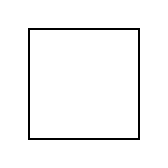
\begin{tikzpicture}[x=1in,y=1in,baseline=0.2in]
    \draw[line width=0.7pt] (0,0) rectangle ++(0.55,0.55);
  \end{tikzpicture}}
\newcommand{\smallblocks}{%
  \par\smallskip
  {\renewcommand{\blkscale}{0.42}\renewcommand{\footnotesize}{\scriptsize}%
  \makebox[\linewidth][c]{\bTri\hfill\bRhombus\hfill\bTrap\hfill\bHex\hfill\bChevron\hfill\bRight\hfill\bKite\hfill\bDart}}\par}
